\section{Резултати}

\subsection*{Генериране на ориентиран граф}

\begin{tabular}{|c|c|c|c|}
\hline
Threads & Time (s) & $S_p$ & $E_p$\\
\hline \hline
1	& 45.29  & 1.0000  & 1.0000 \\
\hline
2	& 22.5   & 2.0129  & 1.0064 \\
\hline
3	& 15.51  & 2.9201  & 0.9734 \\
\hline
4	& 11.04  & 4.1024  & 1.0256 \\
\hline
6	& 7.55   & 5.9987  & 0.9998 \\
\hline
8	& 6.11   & 7.4124  & 0.9266 \\
\hline
12	& 4.06   & 11.1552 & 0.9296 \\
\hline
14	& 3.71   & 12.2075 & 0.8720 \\
\hline
16	& 3.55   & 12.7577 & 0.7974 \\
\hline
20	& 3.28   & 13.8079 & 0.6904 \\
\hline
24	& 2.84   & 15.9472 & 0.6645 \\
\hline
\end{tabular}

\subsection*{Обхождане на графа}

\begin{tabular}{|c|c|c|c|}
\hline
Threads & Time (s) & $S_p$ & $E_p$\\
\hline \hline
1	& 7.16   & 1.0000 & 1.000 \\
\hline
2	& 98.1   & 0.0730 & 0.0365 \\
\hline
3	& 79.93  & 0.0896 & 0.0299 \\
\hline
4	& 59.55  & 0.1202 & 0.0301 \\
\hline
6	& 42.65  & 0.1679 & 0.0280 \\
\hline
8	& 30.67  & 0.2335 & 0.0292 \\
\hline
12	& 28.42  & 0.2519 & 0.0210 \\
\hline
14	& 26.86  & 0.2666 & 0.0190 \\
\hline
16	& 27.3   & 0.2623 & 0.0164 \\
\hline
20	& 25.39  & 0.2820 & 0.0141 \\
\hline
24	& 25.41  & 0.2818 & 0.0117 \\
\hline
\end{tabular}

\subsection*{Финална оценка}

\paragraph*{} Понеже последователния dfs алгоритъм се оказа много по-бърз от паралелния във всички случаи, програмата беше пренаправена да използва паралелното генериране и последователен dfs във всички случаи. Графики на ускорението и ефикасността могат да се видят на фигури \ref{fig::acceleration} и \ref{fig::efficiency}.

\begin{tabular}{|c|c|c|c|}
\hline
Threads & Time (s) & $S_p$ & $E_p$\\
\hline \hline
1 & 52.45 & 1.0000 & 1.0000 \\
\hline
2 & 29.66 & 1.7684 & 0.8842 \\
\hline
3 & 22.67 & 2.3136 & 0.7712 \\
\hline
4 & 18.2 & 2.8819 & 0.7205 \\
\hline
6 & 14.71 & 3.5656 & 0.5943 \\
\hline
8 & 13.27 & 3.9525 & 0.4941 \\
\hline
12 & 11.22 & 4.6747 & 0.3896 \\
\hline
14 & 10.87 & 4.8252 & 0.3447 \\
\hline
16 & 10.71 & 4.8973 & 0.3061 \\
\hline
20 & 10.44 & 5.0239 & 0.2512 \\
\hline
24 & 10 & 5.2450 & 0.2185 \\
\hline
\end{tabular}

\begin{figure}[h]
  \centering
  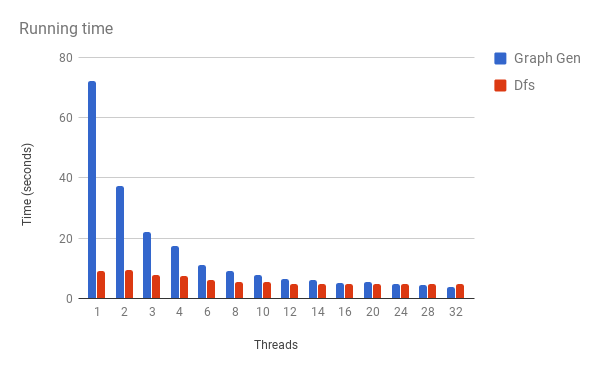
\includegraphics[width=0.8\textwidth]{resources/running_time.png}
  \caption{\label{fig::running_time} Време за изпълнение на отделните части от алгоритъма}
\end{figure}

\begin{figure}[h]
  \centering
  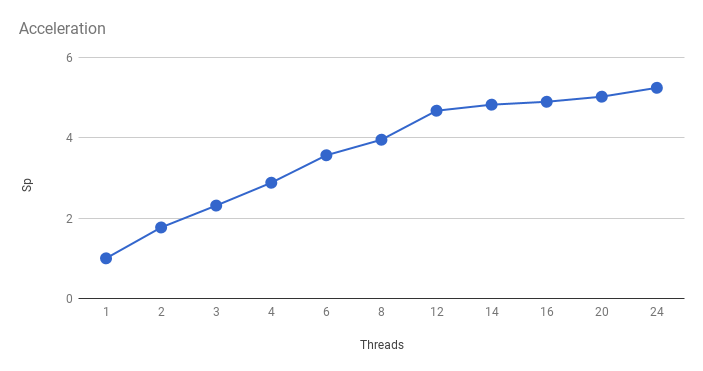
\includegraphics[width=0.8\textwidth]{resources/acceleration.png}
  \caption{\label{fig::acceleration} Графика на ускорението }
\end{figure}

\begin{figure}[h]
  \centering
  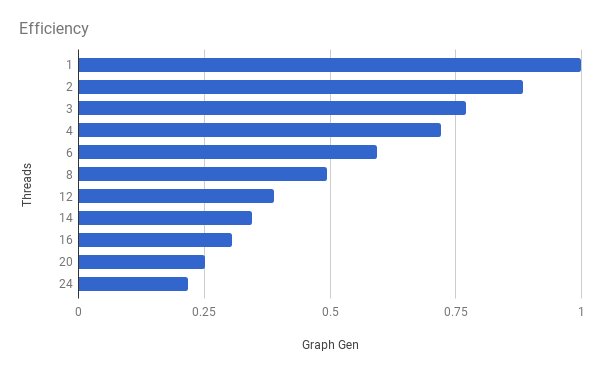
\includegraphics[width=0.8\textwidth]{resources/efficiency.png}
  \caption{\label{fig::efficiency} Графика на ефикасността }
\end{figure}
